\chapter{Latex-Beispiele}
Hier ist eine kleine Sammlung mit Dingen, welche man gern mit Latex anstellt.\par
Dieses Kapitel lässt sich durch eine Einstellung in \emph{settings.tex} verstecken.
Du musst einfach die "`Variable"' \enquote{showExampleChapter} auf \emph{false} setzen.
Das normale Komma in Latex, unterscheidet sich lediglich im Zeichenabstand
vom Dezimalen Komma: 1{,}2 mm. \href{http://google.de}{Siehe Google.}
Oder wie Goethe schon damals sagte: "`Hallo"'\cite[chapter, p.~215]{goethe2016wilhelm}.
Bla bla bla. \parencite[see][p10]{lamport1994latex} Blup \acrlong{gcd} \acrshort{lcm}.
Misc ist die Kurzform für das lateinische Wort Miscellanea und steht
für \emph{verschiedenes}.\cite{wiki:misc}

\section{Grafiken einbinden}

\begin{figure}[ht]
\centering
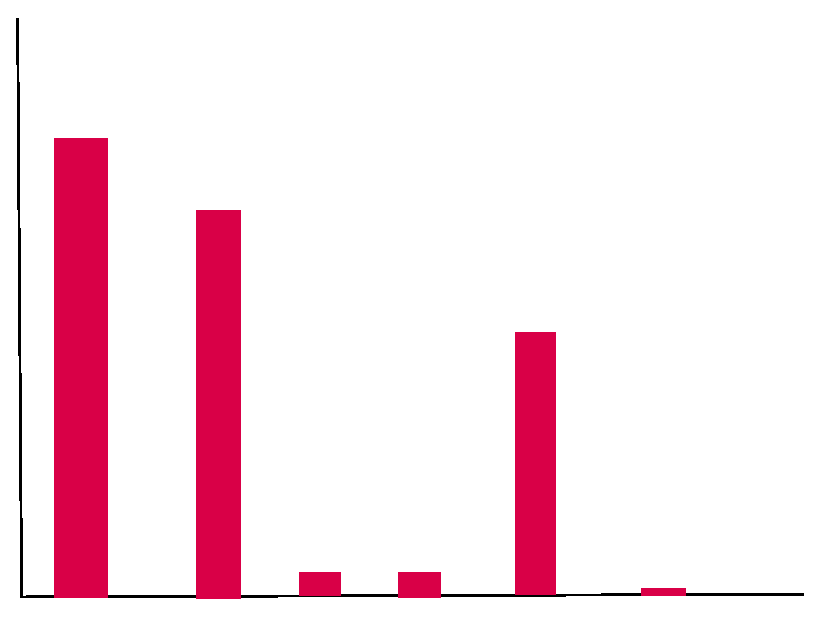
\includegraphics[scale=1.0]{exampleDiagram}
\caption{Das Bild bei scale=1.0}
\label{fig: LogoGross}
\end{figure}

\begin{figure}[ht]
\centering
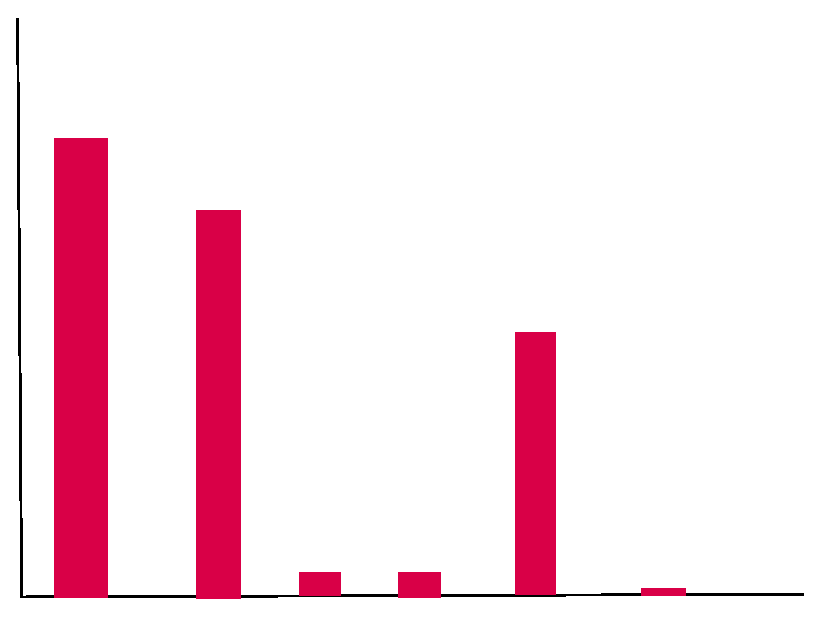
\includegraphics[scale=0.5]{exampleDiagram}
\caption{Das Bild bei scale=0.5}
\label{fig: LogoKleiner}
\end{figure}

\newpage

\section{Listen}

\begin{enumerate}
\item Früchtchen
\begin{enumerate}
\item Äpfel
\item Birnen
\end{enumerate}
\item Orangen
\item Bananen \ldots
\end{enumerate}

\href{https://en.wikibooks.org/wiki/LaTeX/List_Structures}{siehe Wikibooks}

\section{Tabellen}
%%
% Zentrierte Tabelle
%%
\begin{center}
  \begin{tabular}{ | l || c ||| r }
    \hline
    1 & 2 & 3 \\ \hline
    4 & 5 & 6 \\ \hline \hline
    7 & 8 & 9 \\
    \hline
  \end{tabular}
\end{center}

%%
% Tabelle mit Beschriftung
%%
\begin{table}[ht]
\centering
\begin{tabular}{l | l | l}
A & B & C \\
\hline
1 & 2 & 3 \\
4 & 5 & 6
\end{tabular}
\caption{Tabelle mit Beschriftung}
\label{tab:abc}
\end{table}

%%
% Mehrere Tabellen nebeneinander
%%
\begin{table}[ht]
    \begin{subtable}[ht]{0.45\textwidth}
        \centering
        \begin{tabular}{l | l | l}
        Day & Max Temp & Min Temp \\
        \hline \hline
        Mon & 20 & 13\\
        Tue & 22 & 14\\
        Wed & 23 & 12\\
        Thurs & 25 & 13\\
        Fri & 18 & 7\\
        Sat & 15 & 13\\
        Sun & 20 & 13
        \end{tabular}
        \caption{First Week}
        \label{tab:week1}
    \end{subtable}
    \hfill
    \begin{subtable}[ht]{0.45\textwidth}
        \centering
        \begin{tabular}{l | l | l}
        Day & Max Temp & Min Temp \\
        \hline \hline
        Mon & 17 & 11\\
        Tue & 16 & 10\\
        Wed & 14 & 8\\
        Thurs & 12 & 5\\
        Fri & 15 & 7\\
        Sat & 16 & 12\\
        Sun & 15 & 9
        \end{tabular}
        \caption{Second Week}
        \label{tab:week2}
    \end{subtable}
    \caption{Max and min temps recorded in the first two weeks of July}
    \label{tab:temps}
\end{table}

\href{https://en.wikibooks.org/wiki/LaTeX/Tables}{siehe Wikibooks}

\section{Formeln}
Eine Formel wie \( f(x)=x^2 \) kann innerhalb eines Textes stehen.
Komplexere Formeln sollten aber alleine stehen:
\[
  \tan (\alpha) = \frac{a}{c}
\]
\[
  \mathcal S=1=\sqrt{1}=\sqrt[3]{1}=1^{\frac{8}{4}}=\frac{2}{1}\cdot\frac{1}{2}
  = \sum_{i=1}^{1} 1^i
\]

\href{https://en.wikibooks.org/wiki/LaTeX/Mathematics}{siehe Wikibooks}

\section{Zeichnung}
Mit Latex können auch Bilder gezeichnet werden:\\
\setlength{\unitlength}{0.8cm}
\begin{picture}(6,5)
\thicklines
\put(1,0.5){\line(2,1){3}}
\put(4,2){\line(-2,1){2}}
\put(2,3){\line(-2,-5){1}}
\put(0.7,0.3){$A$}
\put(4.05,1.9){$B$}
\put(1.7,3.15){$C$}
\put(3.1,2.5){$a$}
\put(1.2,1.7){$b$}
\put(2.6,1.05){$c$}
\put(0.3,4){$F=\sqrt{s(s-a)(s-b)(s-c)}$}
\put(3.5,0.4){$\displaystyle s:=\frac{a+b+c}{2}$}
\end{picture}
